\section{EXPERIMENTAL RESULTS}\label{sec:4experiment}
In this section, we discuss the experiment methodology and detail the evaluation results.



\subsection{Evaluation Results}
We focus on the detection accuracy about five events, that are body posture, the body rollover, the hand position, the micro body movement and the acoustic events.
%, the classification of micro body movement

\subsubsection{Performance of body posture classification}
To test the detection accuracy of different body postures, we first use the data of User 1 to train the classifier, and this classifier is used for other fourteen persons. We found that training data using only one person's sleeping position has achieved good accuracy, so we currently use only one person's data to train the classifier. In future work, we can also use multiple people's data to expand the sample library. Fig. \ref{fig:posture_zhu} plots the performance across different users. We observe that the posture detection accuracy is consistently high across all users, and it does not show major variations across users. One of the reasons that we know the detection performance of sleeping posture is so good is that the position of the arm in different sleeping positions is specific, which is very helpful for our classification. And we try to consider more arm positions as much as possible.

\begin{figure}[!thbp]
 \centering
 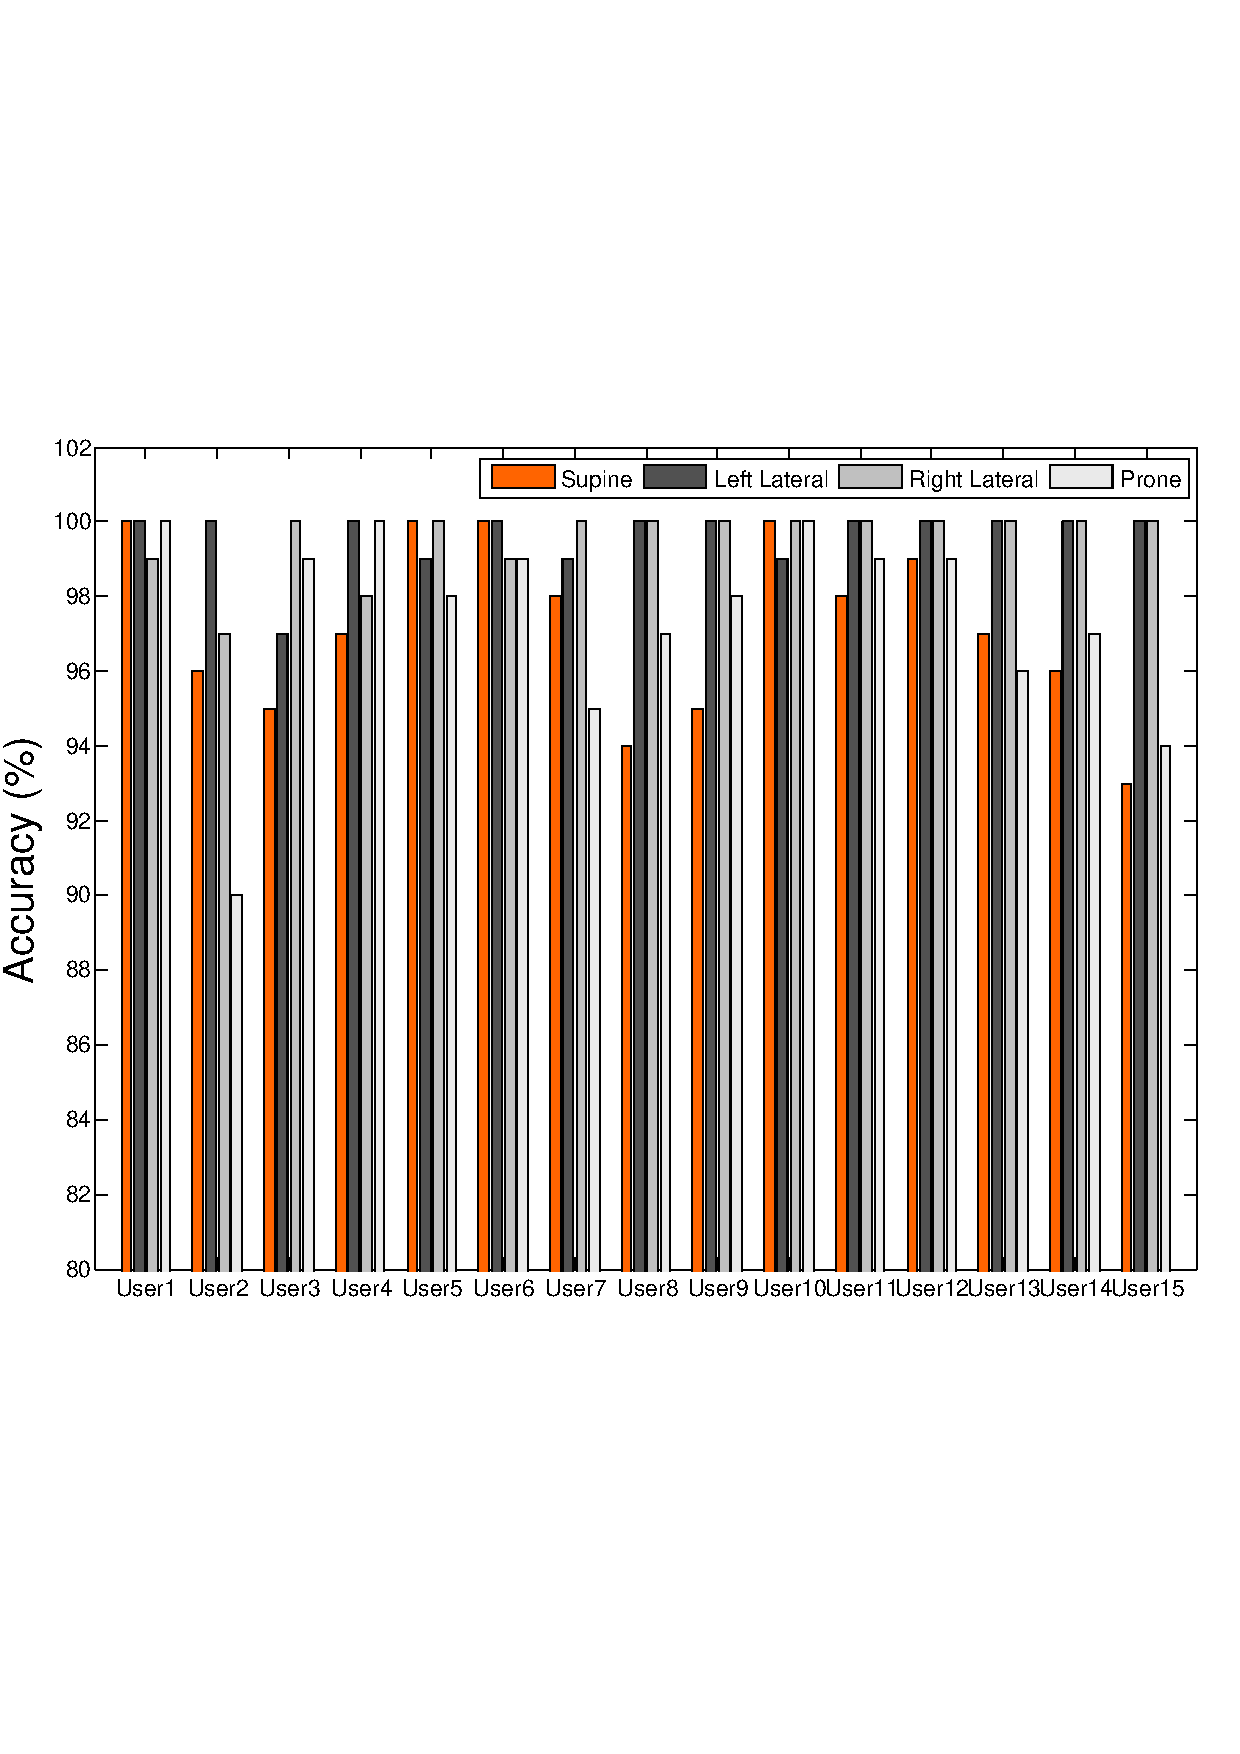
\includegraphics[width=0.67\linewidth]{Figures/posture_zhu.pdf}
 \caption{Detection accuracy of body postures.}\label{fig:posture_zhu}
 \end{figure}

Then to test the overall sleep posture detection performance, we calculate the detection precision and recall across all postures. The result is shown in Table \ref{tab:posture}. The values in blocks are the corresponding numbers of the four types of sleep postures in our testing data. We may find that a small amount of the supine posture are classified as left-sided, possibly due to the fact that the angle features of acceleration when the person is in the supine position with the hand put on the head is closer to the angle features of acceleration when the person is in the left side. And as we can see, the total amount of the prone posture is less than the number of other postures. It suggests that most people are not accustomed to sleep in the prone posture, because it is neither healthy nor comfortable. All in all, Table \ref{tab:posture} shows the outstanding detection performance.

\begin{table}[!thbp]
 \tabcolsep1pt
  \centering  % ������
  %\renewcommand\arraystretch{0.277}
  %\caption{The confusion matrix of body posture classification.}\label{tab:posture}
  %\noindent\makebox{%
%\begin{tabular}{1\textwidth}{ c | c | c | c | c | c | c}
  \renewcommand\arraystretch{0.3}
  \caption{The confusion matrix of body posture classification.}\label{tab:posture}
\begin{tabular}{c| c | c | c | c | c | c}
   \cline{1-7}
   &\multicolumn{1}{ c|}{ }
   & \multicolumn{4}{ c|}{ }\\
   \multirow{2}*{}
&\multicolumn{1}{c|}{\multirow{2}*{{Result}}}
&\multicolumn{4}{c|}{{Prediction}}
& \multirow{4}*{{Recall}} \\
    %&\multicolumn{5}{ c |}{\textbf{\small Prediction}} \\
   % & \multicolumn{5}{ c |}{ } \\
    \cline{3-6}
    & & & & & \\
    \multicolumn{1}{c|}{{}}
    &  \multicolumn{1}{c|}{{}}
    &  \multicolumn{1}{c|}{{Supine}}
    &  \multicolumn{1}{c|}{{Left Lateral}}
    &  \multicolumn{1}{c|}{{Right Lateral}}
    &  \multicolumn{1}{c|}{{Prone}}   \\
    & & & & & \\
     \cline{1-7}
    & & & & & \\
    \multirow{5}{*}{\begin{sideways}{{Groundtruth}}\end{sideways}}
    &   {Supine}   & {\bf{{1182}}}    &   $25$      &   $4$      &   $9$    &   {96.7\%}\\
    & & & & & \\
    \cline{2-7}
    & & & & & \\
   &   {Left Lateral}   &   $6$      &   {\bf{{1292}}}     &   $0$      &   $0$   &   {99.5\%} \\
    & & & & & \\
     \cline{2-7}
    & & & & & \\
    &   {Right Lateral}   &   $7$      &   $0$      &  {\bf{{1275}}}      &   $12$  &   {98.5\%}  \\
    & & & & & \\
     \cline{2-7}
    & & & & & \\
    &   {Prone}   &   $19$      &   $2$      &   $3$      &   {\bf{{567}}}   &   {95.9\%} \\
    & & & & & \\
    \cline{1-7}
    & & & & & \\
    &   {Precision}    &   {97.3 \%}   &   {98.0\%}   &   {99.5\%}   &   {96.4\%}    \\
    & & & & & \\
    \cline{1-7}
   \end{tabular}
\end{table}

\subsubsection{Performance of body rollover counting}
To verify the efficiency of body rollover detection algorithm, we compare the number of body rollover detected by {\systemname} with the groundtruth number recorded by camera. The detection performance is showed in Table \ref{tab:rollver}. We can see from Table 2 that User 3 has an unusually high number of turns, probably trouble falling asleep caused by sleep disorder. For 15 users, the average detection accuracies are all very high, and the least one is still 87\%. Thus our system can accurately distinguish the large hand movement from the body rollover in bed. However, detecting errors in body rollover events will not have a significant impact on our end result, because the division of the sleep stage is a comprehensive consideration of all the features of the sleep stage, such as micro body movement and acoustic events.

\begin{table}[!thbp]
  %\centering  % ������
  \tabcolsep 1pt
  %\arrayrulewidth1pt
  \caption{Detection accuracy of body rollover.}\label{tab:rollver}
   \renewcommand\arraystretch{1.3}{\multirowsetup}{\centering}
        \begin{tabular}{c|ccccccccccccccc}
        \hline
         { User}    & 1& 2  & 3& 4& 5& 6& 7& 8& 9& 10& 11& 12& 13& 14& 15\\
                \hline
               { Groundtruth}  &231&284&348&308&288&301&296&283&293&288&291&279&290&319&286 \\
                \hline
                 { Accuracy} &91\%& 94\% &88\%&93\%&96\%&94\%&87\%&90\% &93\% &94\% &92\% &94\% &89\% &90\% &95\%\\
        \hline
 \end{tabular}
\end{table}

\subsubsection{Performance of hand position recognition}
To test the identification performance of different hand positions, {\systemname} currently only uses the data of User 1 to train the classifier. The classifier for detecting the hand movement trajectory is combined with the detection of periodic signals caused by respiration, then the hand position which is on the chest or abdomen or head can be identified. Fig. \ref{fig:hand_zhu} illustrates the accuracy of hand position across 15 people. As we can see that with just one set of training data, the accuracies for different users are all higher than 87\%. Therefore, our system can achieve a satisfied identification accuracy for different hand positions at a small price. Moreover, we found that at least four persons out of fifteen participants would tend to put their hands on their heads when they sleep in the supine, which is a bad habit for sleep. And other participants' hand are also often placed at these positions of our interest when they are in their supine posture.


\begin{figure}
 \centering
 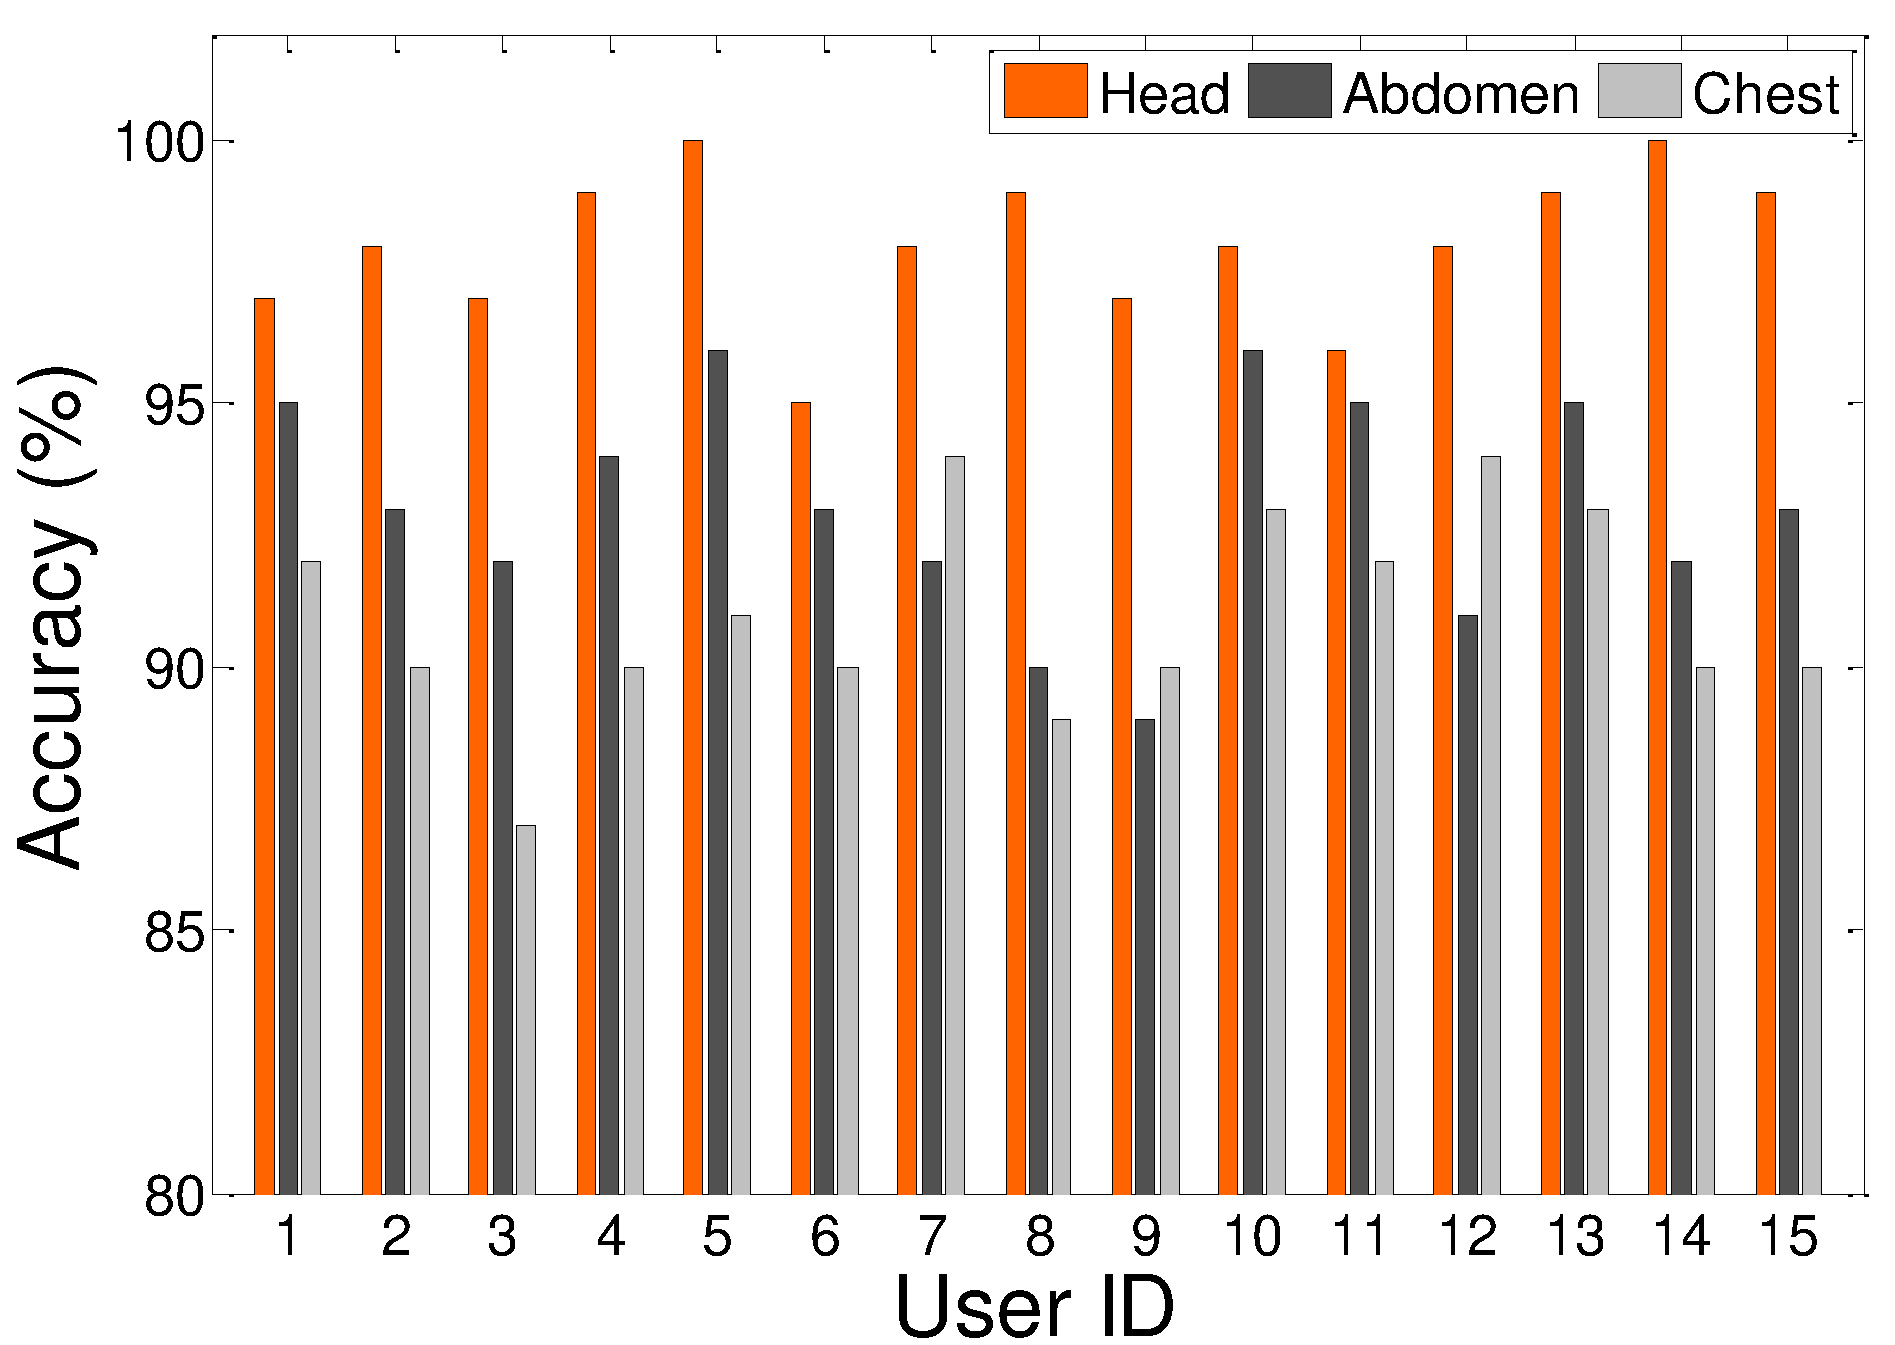
\includegraphics[width=0.67\linewidth]{Figures/handposition_zhu.pdf}
 \caption{Identification accuracy of hand positions}\label{fig:hand_zhu}
\end{figure}




\subsubsection{Performance of micro body movement detection}
To assess the performance of {\systemname}'s detection and classification of user's micro body movements during sleep, we manually mark the types of the micro body movements (hand moving, arm raising, and body trembling) recorded by the camera that occur during sleep. At the same time, we use the accelerometer embedded in a smartphone placed on the bed to record the occurrence of the micro body movements, so as to avoid some movements such as trembling of the body being ignored due to being covered by coverings (such as quilts). And then we combine the two to serve as groundtruth. Fig. \ref{fig:micro_movement_zhu} illustrates the accuracy of the body micro-motion classification across 15 people. We observed that the micro-motion detection accuracy of all users is very close, that is, there will be no major changes between users. And from Fig. \ref{fig:micro_combine}, we can see that even though the worst classification result belongs to the hand movement, the average precision and recall rate still exceed 75\%, and the average accuracy of arm raising and body trembling are 93 \%, 84\%, which indicates that the accuracy of the classification is acceptable. And our purpose of detecting micro body movement is to help us detect the sleep stage, so we are more concerned with body trembling and arm raising, and the poor accuracy of hand moving does not have a significant impact on our end result. The reason for the poor performance of hand movement and body trembling classification may be that we have fewer people to refer to when setting the threshold of the peak value. Specifically, we can further consider more different people in different situations, or set their own thresholds for each person by observing or learning each person's sleep data.


\begin{figure}
\setlength{\abovecaptionskip}{0.cm}
\setlength{\belowcaptionskip}{-0.cm}
 \centering
 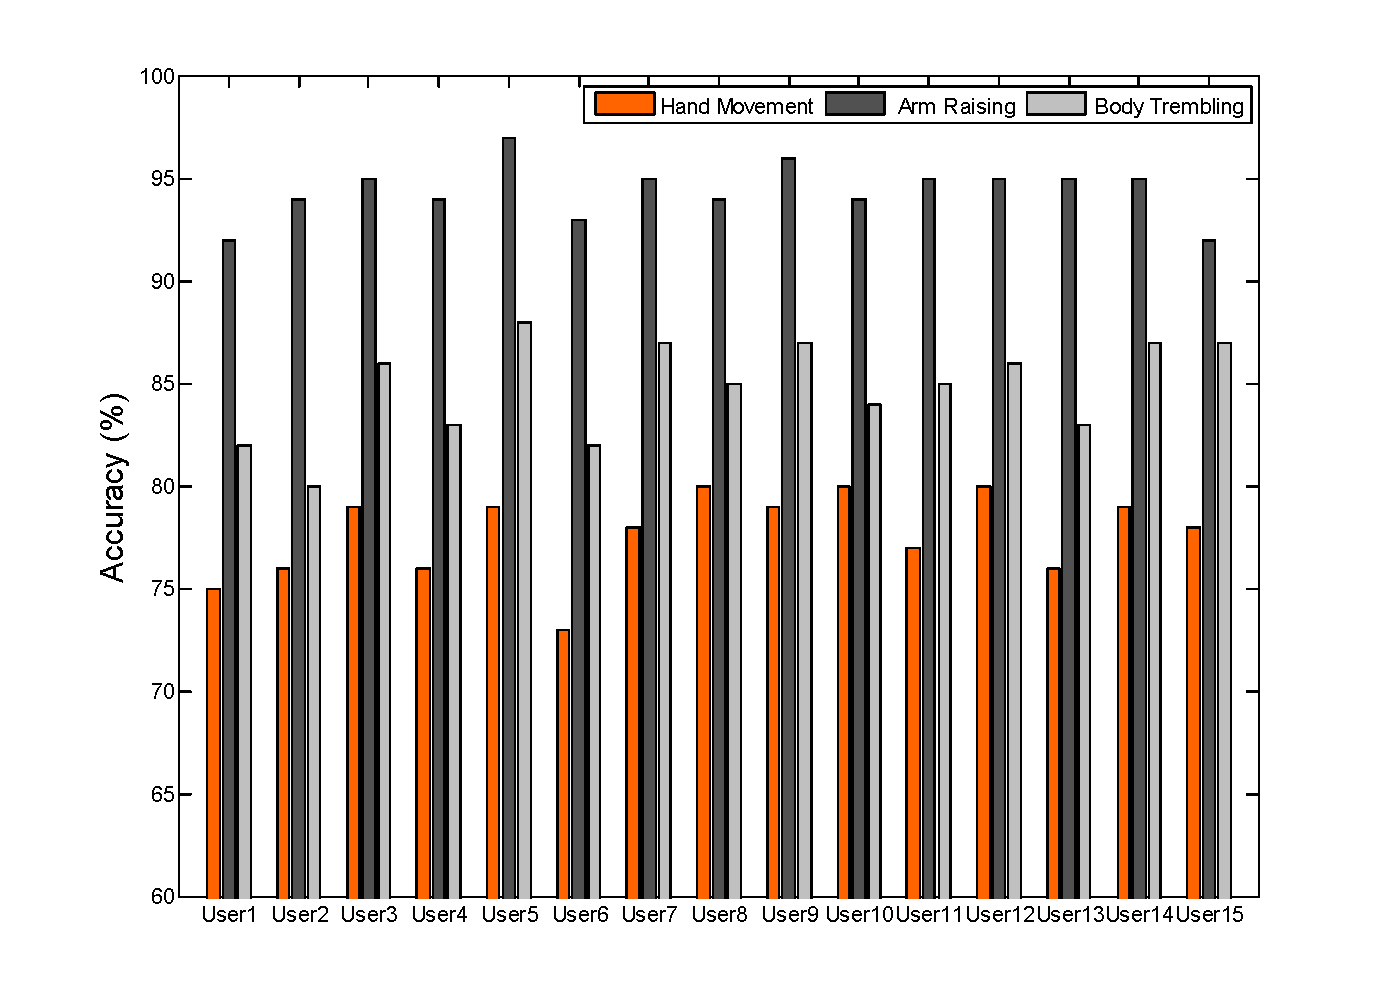
\includegraphics[width=0.67\linewidth]{Figures/micro_movement_zhu.pdf}
 \caption{Detection accuracy of micro body movement.}\label{fig:micro_movement_zhu}
\end{figure}

\begin{figure}
 \centering
   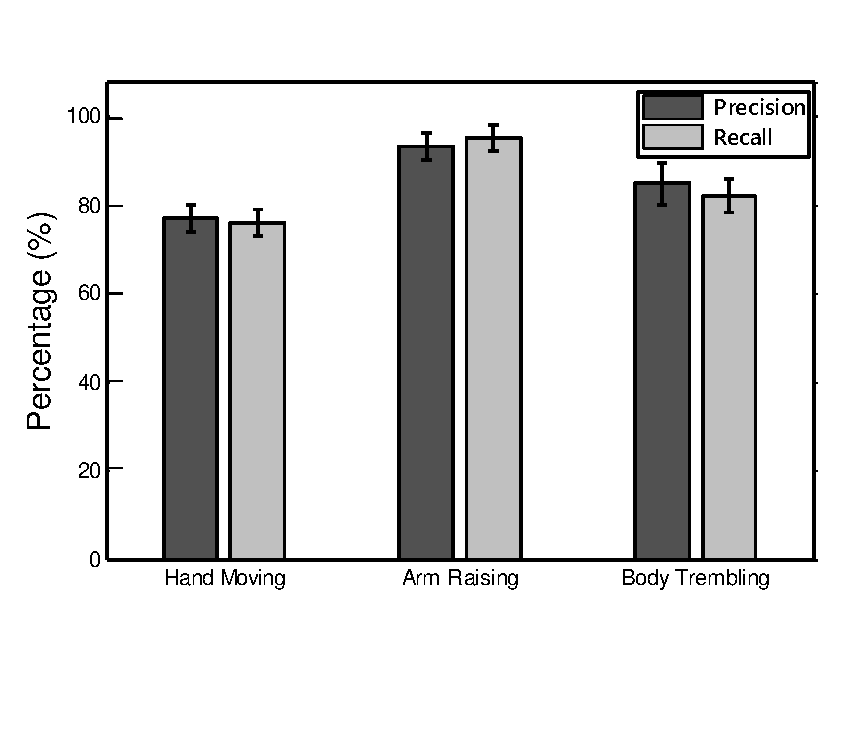
\includegraphics[width=0.47\linewidth]{Figures/micro_combine1.pdf}
 \caption{Micro body movement}\label{fig:micro_combine}
\end{figure}



 \subsubsection{Performance of acoustic events detection}
To study the detection accuracies of different acoustic events, we compare the groundtruth recorded by the camera with the detected results by our system. Table \ref{tab:sound} shows the results across 15 test participants. We can see that the accuracy for cough event is 88.9\%, which is relative lower with regard to other three events. The reason is that different user's cough pattern are different, the pre-defined parameters used in the system does not include all possible patterns. When we train the parameters of the detection algorithm, we only collect 120 sets of nighttime sound data. The data come from 40 (21 males and 19 females) volunteers of different ages (ages 15 to 60) who are prone to snoring, coughing, or somniloquy at night. So in order to further improve the detection accuracy, we can train particular parameters for more different users.

\begin{table}[!thbp]
 \tabcolsep1pt
  \centering  % ������
  \renewcommand\arraystretch{0.3}
  \caption{The confusion matrix of acoustic events detection.}\label{tab:sound}
\begin{tabular}{c| c | c | c | c | c | c}
   \hline
   &\multicolumn{1}{ c|}{ }
   & \multicolumn{4}{ c|}{ }\\
   \multirow{2}*{}
&\multicolumn{1}{c|}{\multirow{2}*{{ Result}}}
&\multicolumn{4}{c|}{{ Prediction}}
& \multirow{4}*{{ Recall}} \\
    %&\multicolumn{5}{ c |}{\textbf{\small Prediction}} \\
   % & \multicolumn{5}{ c |}{ } \\
    \cline{3-6}
    & & & & & \\
    \multicolumn{1}{c|}{{}}
    &  \multicolumn{1}{c|}{{}}
    &  \multicolumn{1}{c|}{{ Snore}}
    &  \multicolumn{1}{c|}{{ Cough}}
    &  \multicolumn{1}{c|}{{ Somniloquy}}
    &  \multicolumn{1}{c|}{{ Other}}   \\
    & & & & & \\
     \cline{1-7}
    & & & & & \\
    \multirow{5}{*}{\begin{sideways}{{ Groundtruth}}\end{sideways}}
    &   { Snore}   & {\bf{{96}}}    &   $0$      &   $0$      &   $9$    &   {91.4\%}\\
    & & & & & \\
    \cline{2-7}
    & & & & & \\
   &   { Cough}   &   $3$      &   {\bf{{64}}}     &   $0$      &   $4$   &   {90.1\%} \\
    & & & & & \\
     \cline{2-7}
    & & & & & \\
    &   { Somniloquy}   &   $0$      &   $3$      &  {\bf{{42}}}      &   $2$  &   {89.4\%}  \\
    & & & & & \\
     \cline{2-7}
    & & & & & \\
    &   { Other}   &   $0$      &   $5$      &   $4$      &   {\bf{{325}}}   &   {97.3\%} \\
    & & & & & \\
    \hline
    & & & & & \\
    &   { Precision}      &   {96.9\%}   &   {88.9\%}   &   {91.3\%}   &   {95.6\%}    \\
    & & & & & \\
    \hline
   \end{tabular}
\end{table}


\subsection{Overall performance}

\subsubsection{Performance of sleep stage detection}
In order to prove that {\systemname} detected these events not only reflect the user's sleep habits, but also can effectively divide the sleep stage in order to assess the quality of sleep, we ask participants to wear Fitbit charge2 \cite{fitbit} during their sleep, and then compare the results of sleep stage detection from Fitbit and those of our system. We regard the detection results of Fitbit as the groundtruth. The average values of precision and recall are shown in Table \ref{tab:sleep stage}. From this table, we can see that although {\systemname} may often make misjudgement between light sleep stage and REM, the overall detection performance of {\systemname} is satisfying.

\begin{table}[!thbp]
 \tabcolsep1pt
  \centering  % ������
  \renewcommand\arraystretch{0.4}
  \caption{ Performance of sleep stage detection.}\label{tab:sleep stage}
\begin{tabular}{c| c | c | c | c | c}
   \hline
   &\multicolumn{1}{ c|}{ }
   & \multicolumn{3}{ c|}{ }\\
   \multirow{2}*{}
&\multicolumn{1}{c|}{\multirow{2}*{{ Result}}}
&\multicolumn{3}{c|}{{ Prediction}}
& \multirow{3}*{{ Recall}} \\
    %&\multicolumn{5}{ c |}{\textbf{\small Prediction}} \\
   % & \multicolumn{5}{ c |}{ } \\
    \cline{3-5}
    & & & & & \\
    \multicolumn{1}{c|}{{}}
    &  \multicolumn{1}{c|}{{}}
    &  \multicolumn{1}{c|}{{ REM}}
    &  \multicolumn{1}{c|}{{ Light Sleep}}
    &  \multicolumn{1}{c|}{{ Deep Sleep}} \\
    & & & & & \\
     \cline{1-6}
    & & & & & \\
    \multirow{4}{*}{\begin{sideways}{{ Groundtruth}}\end{sideways}}
    &   { REM}   & {\bf{{567}}}    &   $244$      &   $47$     &   {70.0\%}\\
    & & & & & \\
     & & & & & \\
    \cline{2-6}
    & & & & & \\
   &   { Light Sleep}   &   $168$      &   {\bf{{607}}}     &   $96$      &   {69.7\%} \\
    & & & & & \\
     \cline{2-6}
    & & & & & \\
    &   { Deep Sleep}   &   $64$      &   $121$      &  {\bf{{197}}}      &   {51.6\%}  \\
    & & & & & \\
     \cline{1-6}
     & & & & & \\
    &   { Precision}      &   {71.0\%}   &   {62.4\%}   &   {58.0\%}   \\
    & & & & & \\
    \hline
   \end{tabular}
\end{table}

\subsubsection{Evaluation on the effect of respiratory amplitude on sleep stage detection}
When we detect the hand's position in the abdomen or chest, we use the magnitude of the acceleration to estimate the amplitude of the respiration. To assess the effectiveness of {\systemname}'s detection of respiration amplitude, we evaluated the performance of the sleep stage test separately in two cases that with considering respiration amplitude and without considering respiration amplitude. And then we can measure the contributions of it for classification of the sleep stage, as we can see in Table \ref{tab:respiratory}. Obviously, When we consider the division of the sleep stage, combining breathing amplitude as a feature with other features, we find that the precision and recall of each sleep stage improve, which proves the effectiveness of our detection of respiration amplitude.

\begin{table} \footnotesize
  \centering  % ������
  \renewcommand\arraystretch{0.3}
  \caption{Evaluation of respiration amplitude contribution}\label{tab:respiratory}
\begin{tabular}{c| c | c | c | c | c | c| c |}
   \cline{2-8}
   &\multicolumn{1}{ c|}{ }
   &\multicolumn{2}{ c|}{ }
   &\multicolumn{2}{ c|}{ }
   & \multicolumn{2}{ c|}{ }\\
   %  \multirow{4}*{}
    &\multicolumn{1}{c|}{}
   &\multicolumn{2}{c|}{\textbf{\scriptsize REM}}
   &\multicolumn{2}{c|}{\textbf{\scriptsize Light Sleep}}
   &\multicolumn{2}{c|}{\textbf{\scriptsize Deep Sleep}} \\
    %&\multicolumn{5}{ c |}{\textbf{\small Prediction}} \\
   % & \multicolumn{5}{ c |}{ } \\
    \cline{2-8}
    & & & & & & &\\
    \multicolumn{1}{c|}{\textbf{}}
    &  \multicolumn{1}{c|}{\textbf{Features}}
    &  \multicolumn{1}{c|}{\scriptsize Precision}
    &  \multicolumn{1}{c|}{\scriptsize Recall}
    &  \multicolumn{1}{c|}{\scriptsize Precision}
    &  \multicolumn{1}{c|}{\scriptsize Recall}
    &  \multicolumn{1}{c|}{\scriptsize Precision}
    &  \multicolumn{1}{c|}{\scriptsize Recall}\\
    & & & & & & &\\
     \cline{2-8}
    & & & & & & &\\
    \multirow{5}{*}
    &   \textbf{\scriptsize Without Respiration Amplitude}   & $62.9\%$    &   $63.4\%$      &   $57.2\%$      &   $63.9\%$    &   $53.3\%$ &  $46.7\%$ \\
    & & & & & & &\\
    \cline{2-8}
    & & & & & & &\\
   &   \textbf{\scriptsize With Respiration Amplitude}   &   $71.0\%$      &   $70.0\%$     &   $62.4\%$      &   $69.7\%$   &   $58.0\%$ &   $51.6\%$ \\
    & & & & & & &\\

   \cline{2-8}

   \end{tabular}
\end{table}

\subsubsection{Performance comparison}
To our knowledge, in the current actigraphy-based work, there is no clear baseline for sleep stage detection performance for us. So we decided to compare {\systemname} with the sleep detection app, Sleep As Android, that has been widely used in the marketplace, in addition, we also considered a comparison with Sleep Hunter \cite{gu2016sleep}. Table \ref{tab:comparison} shows the performance of the sleep stage detection, Sleep As Android can only detect light sleep stage and the deep sleep stage, so we only compared the performance of these two stages.

 \begin{table} \footnotesize
  \centering  % ������
  \renewcommand\arraystretch{0.3}
  \caption{Performance Comparison}\label{tab:comparison}
\begin{tabular}{c| c | c | c | c | c |}
   \cline{2-6}
   &\multicolumn{1}{ c|}{ }
   &\multicolumn{2}{ c|}{ }
   &\multicolumn{2}{ c|}{ }\\
   %  \multirow{4}*{}
    &\multicolumn{1}{c|}{}
   &\multicolumn{2}{c|}{\textbf{\scriptsize Light Sleep}}
   &\multicolumn{2}{c|}{\textbf{\scriptsize Deep Sleep}} \\
    %&\multicolumn{5}{ c |}{\textbf{\small Prediction}} \\
   % & \multicolumn{5}{ c |}{ } \\
    \cline{2-6}
    \multicolumn{1}{c|}{\textbf{}}
    &  \multicolumn{1}{c|}{\diagbox{System}{Stage}}
    &  \multicolumn{1}{c|}{\scriptsize Precision}
    &  \multicolumn{1}{c|}{\scriptsize Recall}
    &  \multicolumn{1}{c|}{\scriptsize Precision}
    &  \multicolumn{1}{c|}{\scriptsize Recall}\\
     \cline{2-6}
    & & & & & \\
    \multirow{5}{*}
    &   \textbf{\scriptsize SleepGuard}   & $62.4\%$    &   $69.7\%$      &   $58.0\%$      &   $51.6$  \\
    & & & & &  \\
    \cline{2-6}
    & & & & & \\
   &   \textbf{\scriptsize Sleep As Android}   &   $27.8\%$      &   $35.4\%$     &   $35.7\%$      &   $50.2\%$   \\
    \cline{2-6}
    & & & & & \\
    &   \textbf{\scriptsize Sleep Hunter}   &   $66.74\%$      &   $66.11\%$     &   $60.00\%$      &   $50.73\%$   \\

   \cline{2-6}

   \end{tabular}
\end{table}

As we can see, {\systemname} can not only perform better on sleep stage detection than Sleep As Android, but also detect one more sleep stage. As for Sleep Hunter, its detection ability is comparable to our system. But our system can provide richer sleep data for users and take more factors that affect sleep quality into consideration, making users understand their sleep more easily and improve their sleep quality more effectively. Further, we show our superior in function comapared with other similar sleep detection products, including Sleep As Android, Sleep Hunter, sleepMonitor \cite{sleepmonitor}, Sleeptracker \cite{sleeptracker}, Fitbit, isleep \cite{hao2013isleep}, Jawbone \cite{Jawbone},ubiSleep \cite{pombo2016ubisleep}, in Table \ref{tab:function}. As we have shown, {\systemname} can detect a wider range of sleep events to provide a better user experience.

\begin{table*}\scriptsize
\setlength{\abovecaptionskip}{0.8pt}
  \centering  % ������
  \tabcolsep10pt
  \arrayrulewidth1pt
  \caption{Systems for support sleep}\label{tab:function}
  \renewcommand{\multirowsetup}{\centering}
  \noindent\makebox[\textwidth]{%
        \begin{tabularx}{1.0\textwidth}{|c|c|c|c|c|c|c|}
        \cline{1-7}
        \multicolumn{1}{|c|}{\multirow{2}*{\textbf{\scriptsize System}}}
        &\multicolumn{6}{c|}{\textbf{ \scriptsize Detected Events}} \\
         \cline{2-7}
    &  \multicolumn{1}{c|}{\textbf{ \scriptsize Heart Rate }}
    &  \multicolumn{1}{c|}{\textbf{ \scriptsize Acoustic Event }}
    &  \multicolumn{1}{c|}{\textbf{ \scriptsize Sleep Posture }}
     &  \multicolumn{1}{c|}{\textbf{ \scriptsize body Movement }}
      &  \multicolumn{1}{c|}{\textbf{ \scriptsize hand position}}
       &  \multicolumn{1}{c|}{\textbf{ \scriptsize Sleep Stage}} \\
        \cline{1-7}
        \multirow{7}{2cm}
        {\textbf{SleepGuard\\Sleep as Android\\Sleep Hunter\\SleepMonitor\\Sleeptracker\\isleep \\Fitbit\\Jawbone\\ ubiSleep } }
        & &$\checkmark$ & $\checkmark$ &  $\checkmark$  &$\checkmark$ &$\checkmark$\\
        & &$\checkmark$ & & & &$\checkmark$\\
        & & $\checkmark$& &$\checkmark$ & &$\checkmark$\\
        & & & $\checkmark$ & & &\\
        &$\checkmark$ & & & & &$\checkmark$\\
         & &$\checkmark$ &   &$\checkmark$ & &\\
         &$\checkmark$ & & & & &$\checkmark$ \\
        & & & & & &$\checkmark$ \\
        & $\checkmark$&$\checkmark$ & & & &\\
        \cline{1-7}
 \end{tabularx}}
\end{table*}

\subsubsection{User survey}
In order to evaluate whether {\systemname} can provide help in the assessment of sleep quality and has a good user experience, we conducted a user survey of 15 volunteers participating in our experiments. In our survey, we asked participants to fill out our questionnaire based on PSQI \cite{carpenter1998psychometric} every morning during the experiment, in order to get their subjective feeling of sleep quality and use experience for our system. We use the following questions in our survey, which includes:
\begin{enumerate}
  \item Subjective sleep quality (5 levels, 1 for excellent and 5 for worst)
  \item Sleep duration
  \item Sleep disturbances
  \item Daytime dysfunction
\end{enumerate}

The statistical results of the assessment of sleep quality of 15 individuals are shown in Fig. \ref{fig:quality}, the figure on the right is the result of {\systemname} statistics, and the figure on the left is based on questionnaire subjective sleep quality. We can see the result is satisfactory and representative to some extent. In addition, we also ask whether users are interested in these events, such as sleep posture, hand position, which detected by {\systemname}. 80\% of participants believe that the detection of sleep posture is very necessary, showing their sleep posture can not only help people to avoid health problems caused by long-term improper sleeping posture, but also help us find out the reasons for the next day's physical discomfort, such as dizziness, muscle soreness may be due to improper sleeping position. 60\% of the participants thought it useful to detect their hand position in the supine position and even one user mentioned that he did often have nightmares and that he found his hands were often placed on his chest. And {\systemname} was able to remind him to avoid such a hand position when sleeping. However, only 20\% of them think it is necessary to calculate the number of body rollover, but the detection of body rollover is very useful in the division of sleep stage.

\begin{figure}
 \centering
 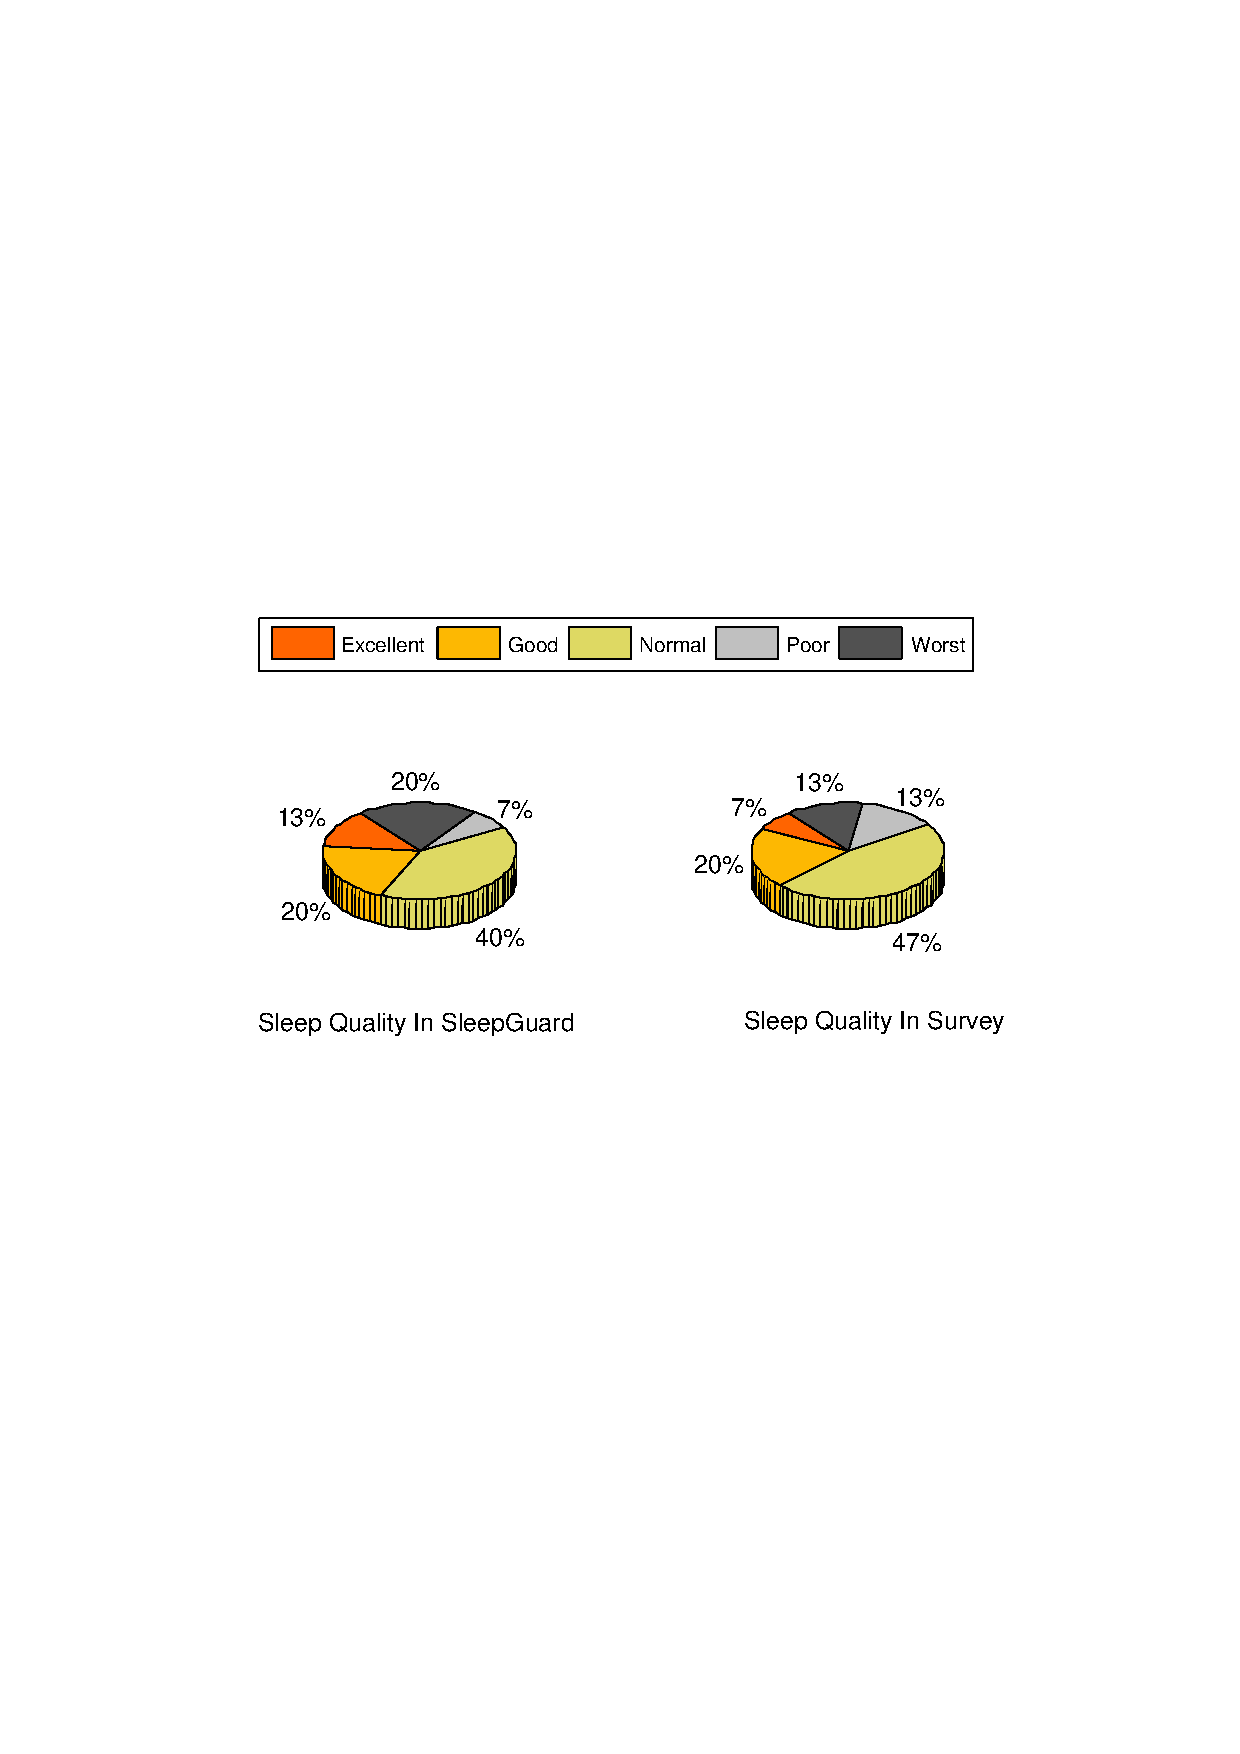
\includegraphics[width=0.77\linewidth]{Figures/quality.pdf}
 \caption{Participants' sleep quality distribution}\label{fig:quality}
\end{figure}
